\documentclass[a4paper,10pt]{article}

\usepackage{color}
\usepackage{xcolor}
\usepackage{tikz}
\usepackage{amsmath}
\usepackage{amssymb}
\usepackage{amsthm}
\usepackage{graphicx}
\usepackage{mathtools}
\usepackage{wrapfig}
\usepackage{multirow}
\usepackage{comment}
\usepackage{natbib}
%\usepackage{float}
\usepackage{appendix}
\usepackage{subfig}
\usepackage{enumitem}
\usepackage{newfloat}
\usepackage[utf8]{inputenc}
\usepackage{floatrow}
\usepackage{bm}
\usepackage{geometry}

\geometry{a4paper,left=10mm,right=10mm}

\usetikzlibrary{calc}
\usetikzlibrary{fit}
\usetikzlibrary{decorations.shapes,shapes.misc,calc, positioning, hobby, backgrounds}

\tikzset{decorate sep/.style 2 args=
{decorate,decoration={shape backgrounds,shape=circle,shape size=#1,shape sep=#2}}}

%\DeclarePairedDelimiter{\floor}{\lfloor}{\rightfloor}
%\DeclarePairedDelimiter{\ceil}{\lceil}{\rceil}

\newcommand{\halflength}{\ensuremath{\floor{\frac{m}{2}}}}
\newcommand{\floor}[1]{\left \lfloor #1 \right \rfloor}
\newcommand{\ceil}[1]{\left \lceil #1 \right \rceil}

\newtheorem{theorem}{Theorem}[section]
\newtheorem{corollary}[theorem]{Corollary}
\newtheorem{lemma}[theorem]{Lemma}

\theoremstyle{definition}
\newtheorem{definition}[theorem]{Definition}

\theoremstyle{definition}
\newtheorem{example}[theorem]{Example}
 
\theoremstyle{remark}
\newtheorem*{remark}{Remark}

\theoremstyle{definition}
\newtheorem*{note}{Note}

\DeclareFloatingEnvironment[fileext=los,
    listname={List of Example Figures},
    name=Example Figure,
    placement=tbhp,
    within=section,]{examplefigure}

\DeclareFloatingEnvironment[fileext=los,
    listname={List of myFigures},
    name=Figure,
    placement=tbhp,
    within=section,]{myfigure}      

\title{A graph Patrol Problem with a random attacker and an observable patroller}
\date{\today}
\author{Thomas Lowbridge \\ School of Mathematical Sciences \\ University of Nottingham}

\bibliographystyle{plain}

\begin{document}

\pagestyle{empty}
{
  \renewcommand{\thispagestyle}[1]{}
  \maketitle
  \tableofcontents  
}
\clearpage
\pagestyle{plain}


\setlength{\parindent}{0pt}
\setlength{\parskip}{1em}

\newpage
\pagenumbering{arabic}
\section{Introduction to a random attacker patroller game with observation}
The model has a graph, $Q=(N,E)$, with a set of nodes labeled $1$ to $n$, $N=\{1,...,n \}$, and a set of edges linking these nodes. The adjacency matrix $a=(a_{i,j})_{i,j \in N}$, has $a_{i,j}=1$ if $i$ and $j$ are adjacent and $a_{i,j}=0$ if they are not adjacent. By definition we will use $a_{i,i}=1 \quad \forall i \in N$.


An attacker has some attack time for node $i$, called $X_{i}$ and chooses to attack node $i$ with some probability, $p_{i}$. The attackers arrive according to some Poisson process with rate $\Lambda$, so by Poisson thinning they arrive at node $i$ according to a Poisson process with rate $\lambda_{i}=\Lambda p_{i}$.

The patroller, uses some walk (with possible waiting) to patrol the graph.We assume that a patrollers walk is able to capture all attacks that have already begun, but not completed. But unlike the `normal' setting the past unit time, the attackers do not start their attacks and instead will wait for the patroller to leave. Each missed attack at node $i$ inccures a cost of $c_{i}$ to the patroller.

We can formulate the state space, as the delineation of separate nodes. $\Omega= \{ (\bm{s},\bm{v})= \quad | \quad s_{i}=1,2,... , v_{i}=0,1,2,... \quad \forall i \in N \}$. Where $\bm{s}=(s_{1},...,s_{n})$ has each $s_{i}$ represent the number of time periods since the last visit for that node $i$ and $\bm{v}=(v_{1},...,v_{n})$ has each $v_{i}$ represent the number of attackers present in the last time period when the node $i$ was last visited (i.e The number of attackers known to be beginning their attack $s_{i}$ time ago at node $i$).

\begin{myfigure}
\begin{center}
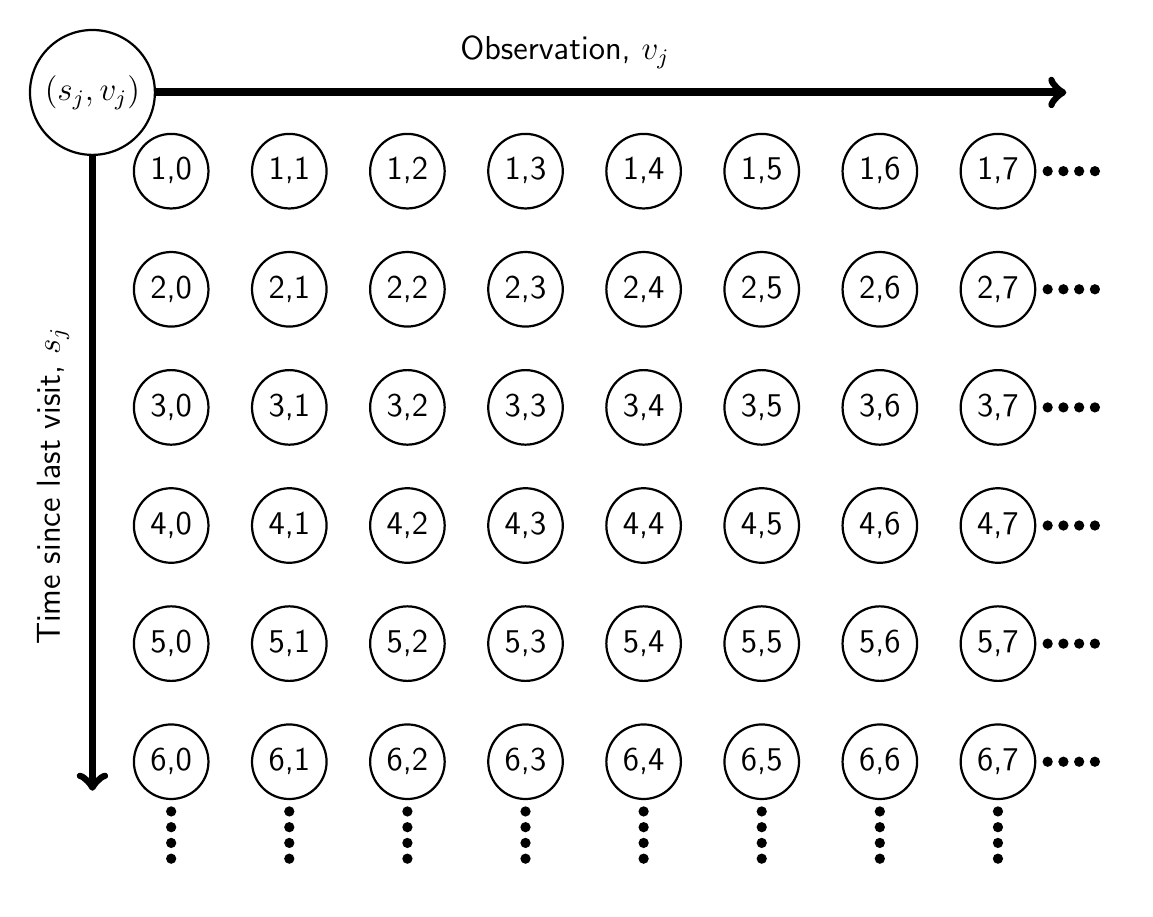
\begin{tikzpicture}[-,auto,node distance=1cm,
                    thick,main node/.style={circle,fill=white,draw,font=\sffamily\large,minimum size=0.5cm}]
 \foreach \x in {0,...,7}
    \foreach \y in {0,...,5} 
       {\pgfmathtruncatemacro{\label}{\x - 5 *  \y +21}
        \pgfmathtruncatemacro{\v}{\x}
        \pgfmathtruncatemacro{\s}{6-\y}
       \node [main node]  (\x\y) at (1.5*\x,1.5*\y) {\s,\v};} 

\node (XaxisLeft) [shift={(-0.5,1)}] at (05) {};
\node (XaxisRight) [shift={(1,1)}] at (75) {};

\node (YaxisBottom) [shift={(-1,-0.5)}] at (00) {};
\node (YaxisTop) [shift={(-1,1)}] at (05) {};

\draw[->,line width=1mm] (XaxisLeft)--(XaxisRight);
\draw[->,line width=1mm] (YaxisTop)--(YaxisBottom);

\node[font=\sffamily\large] (OLabel) [shift={(0.5,1.5)}] at (35) {Observation, $v_{j}$};
\node[font=\sffamily\large] (SLabel) [shift={(-1.5,0.5)}] at (02) {\rotatebox{90}{Time since last visit, $s_{j}$}};

\node[main node] (Example) [shift={(-1,1)}] at (05) {$(s_{j},v_{j})$};

\foreach \y in {0,...,5}
{\node (DottedStart\y) [shift={(0.5,0)}] at (7\y) {};
 \node (DottedEnd\y) [shift={(1.5,0)}] at (7\y) {};
 \draw[decorate sep={1mm}{2mm},fill] (DottedStart\y)--(DottedEnd\y);}
 
\foreach \x in {0,...,7}
{\node (\x DottedStart) [shift={(0,-0.5)}] at (\x0) {};
 \node (\x DottedEnd) [shift={(0,-1.5)}] at (\x0) {};
 \draw[decorate sep={1mm}{2mm},fill] (\x DottedStart)--(\x DottedEnd);
} 
\end{tikzpicture}
\end{center}
\caption{State space diagram}
\end{myfigure}

The $s_{i}$ increment by $1$ if the node is not visited upon each action, or if the node is visited reset to $s_{i}=1$. The $v_{i}$ do not change for nodes not visited, when a node is visited, the $v_{i}$ `reset' according to the Poisson distribution $Po(\lambda_{i} \times 1)=Po(\lambda)$. Due to $s_{i}=1$ if and only if the patroller is currently at this node, we will use $l(\bm{s})=\arg\min\limits_{i \in N} s_{i}$ to represent the current node.

As the future of the process is independent of its past, the process can be formulated as a Markov decision process(MDP), where at the end of the period, the patroller chooses which adjacent node to visit. Thus the action space is $\mathcal{A}=\{ j \, | \, a_{l(\bm{s}),j}=1 \}$, with a deterministic, stationary policy, $\pi: \Omega \rightarrow \mathcal{A}$.

The transitions of the MDP aren't entirely deterministic, $\bm{s}$ is purely deterministic, but $\bm{v}$ is partially probabilistic. In state $(\bm{s},\bm{v})$ with the decision to visit node $i \in \mathcal{A}$, then the state will transition to $(\widetilde{\bm{s}},\widetilde{\bm{v}})$ where $\widetilde{s}_{j}=s_{j}+1$ if $j \neq i$ and $\widetilde{s}_{j}=1$ if $j=i$ and $\widetilde{v}_{j}=o_{j}$ if $j \neq i$ and $v_{j} \sim Po(\lambda)$ if $j=i$.

To write down the cost function, which is dependent on the state $(\bm{s},\bm{v})$ and the action to visit node $i$ chosen, we will look at the expected cost of incurred at all nodes and sum these costs for the next time period.

\begin{align}
C_{j}(\bm{s},\bm{v},i)&= \begin{cases}
c_{j} \lambda_{j} \int_{0}^{s_{j}} P(t-1<X_{j} \leq t) dt +v_{j}P(0<X_{j} \leq s_{j})  \text{ for } i \neq j \\
c_{j} \lambda_{j} \int_{0}^{s_{j}-1} P(t-1<X_{j} \leq t) dt +v_{j}P(0<X_{j} \leq s_{j})  \text{ for } i=j \\
\end{cases}
 \nonumber \\
&= \begin{cases}
c_{j} \lambda_{j} \int_{s_{j}-1}^{s_{j}} P(X_{j} \leq t) dt +v_{j}P(X_{j} \leq s_{j}) \text{ for } i \neq j \\
c_{j} \lambda_{j} \int_{s_{j}-2}^{s_{j}-1} P(X_{j} \leq t) dt +v_{j}P(X_{j} \leq s_{j})   \text{ for } i=j \\
\end{cases} 
\end{align}
   
With $C(\bm{s},\bm{v},i)=\sum\limits_{j=1}^{n} C_{j}(\bm{s},\bm{v},i)$ being the cost function for the MDP.

We will now make the assumptions that $X_{j}$ is bounded by $B_{j}$ and that instead of using $Po(\lambda)$ for the observation transition and placing a bound on this Poisson distribution, named $b_{j}$, so we are now drawing from a truncated Poisson distribtion, henceforth called $TPo(\lambda,b_{j})$. Then we can immediately say that the $o_{j} \leq b_{j}$ state is finite and the state $s_{j}$ has the same cost function for $s_{j} \geq B_{j}+2$ and hence we will restrict our space to this. So our modified transition is $\widetilde{s_{j}}=\min(s_{j}+1,B_{j}+2)$ if $j \neq i$ and $\widetilde{s_{j}}=1$ if $i=j$. $\widetilde{v_{j}}=v_{j}$ if $i \neq j$ and $v_{j} \sim TPo(\lambda,b_{j})$ if $i=j$.

The truncated Poisson distribution, $TPo(\lambda,b)$ acts like normal Poisson for any value not equal to $b$, with the tails probability stored at $b$. That is $P(TPo(\lambda,b)=i)=\begin{cases}
P(Po(\lambda)=i) \text{ If } i \neq b \\
P(Po(\lambda) \geq b) \text{ If } i=b \\
0 \text{ Otherwise}
\end{cases}$

\begin{myfigure}
\begin{center}
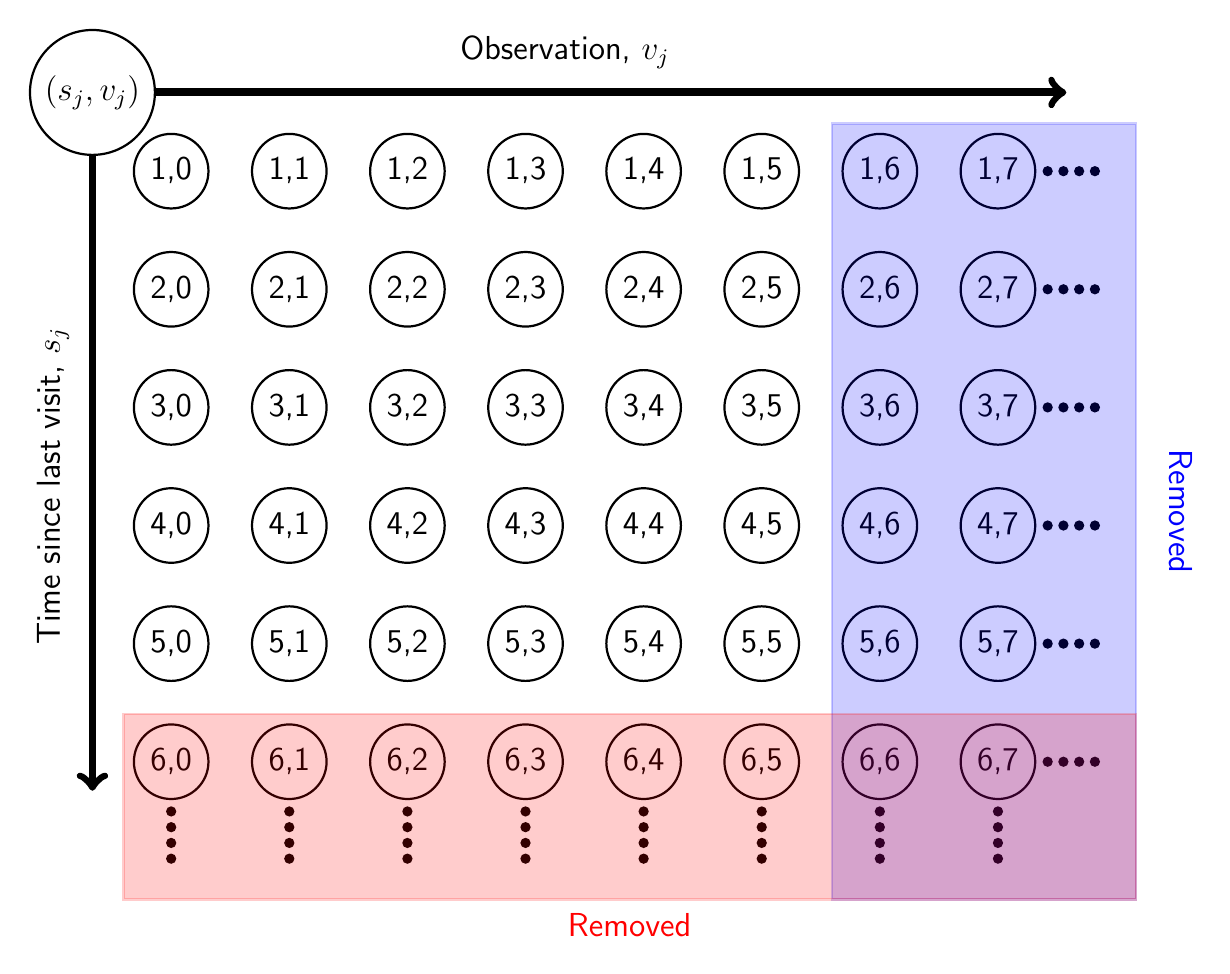
\begin{tikzpicture}[-,auto,node distance=1cm,
                    thick,main node/.style={circle,fill=white,draw,font=\sffamily\large,minimum size=0.5cm}]
 \foreach \x in {0,...,7}
    \foreach \y in {0,...,5} 
       {\pgfmathtruncatemacro{\label}{\x - 5 *  \y +21}
        \pgfmathtruncatemacro{\v}{\x}
        \pgfmathtruncatemacro{\s}{6-\y}
       \node [main node]  (\x\y) at (1.5*\x,1.5*\y) {\s,\v};} 

\node (XaxisLeft) [shift={(-0.5,1)}] at (05) {};
\node (XaxisRight) [shift={(1,1)}] at (75) {};

\node (YaxisBottom) [shift={(-1,-0.5)}] at (00) {};
\node (YaxisTop) [shift={(-1,1)}] at (05) {};

\draw[->,line width=1mm] (XaxisLeft)--(XaxisRight);
\draw[->,line width=1mm] (YaxisTop)--(YaxisBottom);

\node[font=\sffamily\large] (OLabel) [shift={(0.5,1.5)}] at (35) {Observation, $v_{j}$};
\node[font=\sffamily\large] (SLabel) [shift={(-1.5,0.5)}] at (02) {\rotatebox{90}{Time since last visit, $s_{j}$}};

\node[main node] (Example) [shift={(-1,1)}] at (05) {$(s_{j},v_{j})$};

\foreach \y in {0,...,5}
{\node (DottedStart\y) [shift={(0.5,0)}] at (7\y) {};
 \node (DottedEnd\y) [shift={(1.5,0)}] at (7\y) {};
 \draw[decorate sep={1mm}{2mm},fill] (DottedStart\y)--(DottedEnd\y);}
 
\foreach \x in {0,...,7}
{\node (\x DottedStart) [shift={(0,-0.5)}] at (\x0) {};
 \node (\x DottedEnd) [shift={(0,-1.5)}] at (\x0) {};
 \draw[decorate sep={1mm}{2mm},fill] (\x DottedStart)--(\x DottedEnd);
}

\node (Box1) [draw,thick,fit=(65) (60) (DottedEnd5) (DottedEnd0) (6DottedEnd) (7DottedEnd),fill,blue,opacity=0.2] {};

\node (Box2) [draw,thick,fit=(00) (70)(DottedEnd0) (0DottedEnd) (7DottedEnd),fill,red,opacity=0.2] {};

\node[font=\sffamily\large,color=blue] (Box1Text) [shift={(2.5,0)}] at (Box1) {\rotatebox{270}{Removed}};

\node[font=\sffamily\large,color=red] (Box2Text) [shift={(0,-1.5)}] at (Box2) {Removed};           

\end{tikzpicture}
\end{center}
\caption{State space diagram, with \textcolor{blue}{$b_{j}=5$} and \textcolor{red}{$B_{j}=4$}}
\end{myfigure}

Further reduction is possible as if $X_{j} \leq B_{j}$ then any observations $v_{j}$ which started $s_{j}$ time units ago is bound to have finished if $s_{j} \geq B_{j}+1$. So our new state space is further reduced to having only $(\floor{B_{j}}+1,0)$ when $s_{j}=\floor{B_{j}}+1$.

So $\Omega= \{ (\bm{s},\bm{v}) | s_{i}=1,2,..,\floor{B_{i}}+1 , v_{i}=1,...,b_{i} \, \forall i \in N \} \cup \{(\floor{B_{j}}+2,0) \}$.

\begin{myfigure}
\begin{center}
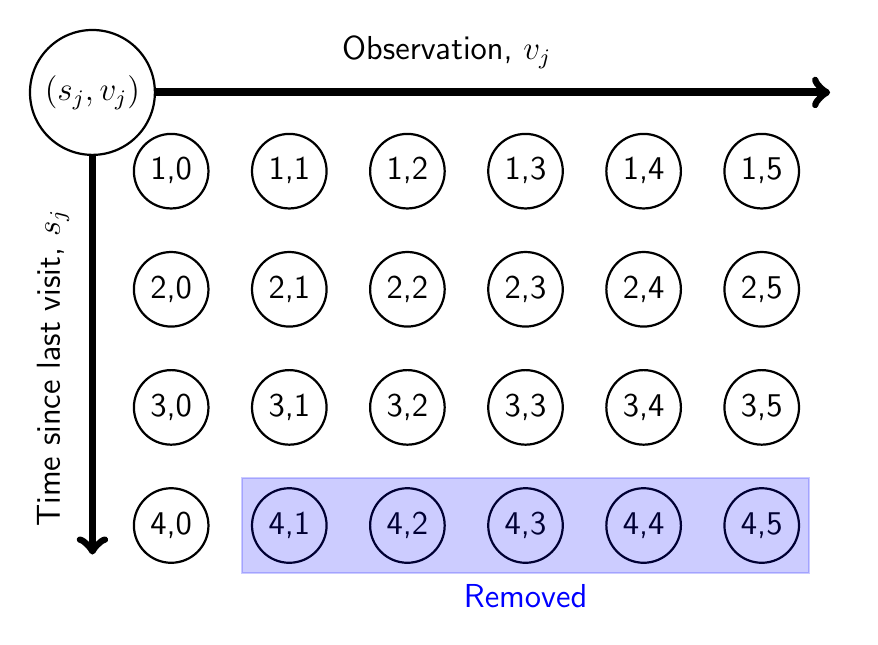
\begin{tikzpicture}[-,auto,node distance=1cm,
                    thick,main node/.style={circle,fill=white,draw,font=\sffamily\large,minimum size=0.5cm}]
 \foreach \x in {0,...,5}
    \foreach \y in {0,...,3} 
       {\pgfmathtruncatemacro{\label}{\x - 5 *  \y +21}
        \pgfmathtruncatemacro{\v}{\x}
        \pgfmathtruncatemacro{\s}{4-\y}
       \node [main node]  (\x\y) at (1.5*\x,1.5*\y) {\s,\v};} 

\node (XaxisLeft) [shift={(-0.5,1)}] at (03) {};
\node (XaxisRight) [shift={(1,1)}] at (53) {};

\node (YaxisBottom) [shift={(-1,-0.5)}] at (00) {};
\node (YaxisTop) [shift={(-1,1)}] at (03) {};

\draw[->,line width=1mm] (XaxisLeft)--(XaxisRight);
\draw[->,line width=1mm] (YaxisTop)--(YaxisBottom);

\node[font=\sffamily\large] (OLabel) [shift={(0.5,1.5)}] at (23) {Observation, $v_{j}$};
\node[font=\sffamily\large] (SLabel) [shift={(-1.5,0.5)}] at (01) {\rotatebox{90}{Time since last visit, $s_{j}$}};

\node[main node] (Example) [shift={(-1,1)}] at (03) {$(s_{j},v_{j})$};

\node (Box1) [draw,thick,fit=(10) (50),fill,blue,opacity=0.2] {};        

\node[font=\sffamily\large,color=blue] (Box1Text) [shift={(0,-0.9)}] at (Box1) {Removed};

\end{tikzpicture}
\end{center}
\caption{State space diagram, with $b_{j}=5$ and $B_{j}=4$ and further reduction}
\end{myfigure}

With further modified transitions that if $s_{j}=\floor{B_{j}}+1$ then $\widetilde{v_{j}}=0$ for $i \neq j$. 

Now our state space and action space are finite we need only consider deterministic, stationary policies. Applying such a policy generates a sequence of states under a given policy $\pi$, namely $\{\psi_{\pi}^{k}(\bm{s}_{0},\bm{o}_{0}), k=0,1,2,... \}$. However we are not guaranteed to every have a regenerating process when the same node is visited due to the unpredictable nature of $o_{i} \sim TPo(\lambda,b_{i})$. Unless $b_{i}=0 \quad \forall i \in N$ then we have removed the probabilistic nature of $v_{i}$'s transition. We will not focus on the special case of $b_{i}=0 \quad \forall i \in N$ but it is shown how to develop a index for the single node problem in Appendix \ref{Observations are always zero}.

\begin{note}
There may be a problem with having a non-deterministic attack time, as this may cause the observable attacker behaviour to no longer take the form of $(\bm{s},\bm{v})$ but the patroller may have other information such as visiting early may mean if they caught less than expected then some in the observed section exist, so a full history could be recorded. However we will not deal with this and assume once a node is visited its last observation is lost and the system is rest???
\end{note}

\section{Single node problem}
Focusing on the problem of a single nodes and stripping off the index, $i$, for the nodes. This problem has a visiting cost, $\omega>0$ and we are looking to minimize the long run cost of the system.

\section{Deterministic Attack time}
Consider the case where $X=x$, where $x$ is a constant (So $B=x$). Then we can further reduce the state space, as we choosing to visit later rather than earlier (as long as its not too late) allows us to possibly catch more (as we know when the attacks can start to finish). So we limit the state space with non-zero observed attackers to only have $s_{j}=\floor{B}+1$, as visiting at then gets any attacks caught when visiting at any $s_{j} < \floor{B}+1$.

So in the deterministic case $\Omega= \{(\floor{B}+1,v) \, | \, v=0,1,...,b \} \cup \{(\floor{B}+2,0) \}$.

\begin{myfigure}
\begin{center}
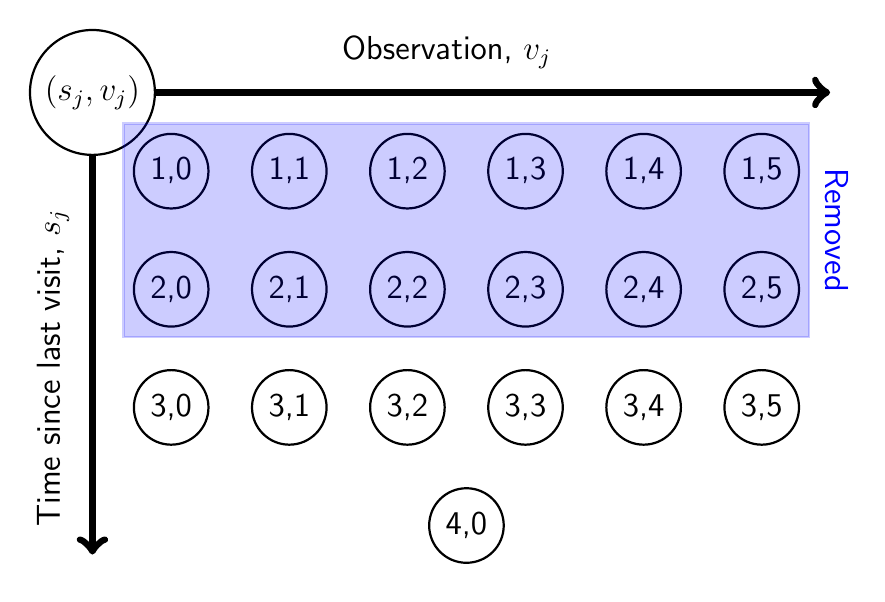
\begin{tikzpicture}[-,auto,node distance=1cm,
                    thick,main node/.style={circle,fill=white,draw,font=\sffamily\large,minimum size=0.5cm}]
 \foreach \x in {0,...,5}
    \foreach \y in {0,...,2} 
       {\pgfmathtruncatemacro{\label}{\x - 5 *  \y +21}
        \pgfmathtruncatemacro{\v}{\x}
        \pgfmathtruncatemacro{\s}{3-\y}
       \node [main node]  (\x\y) at (1.5*\x,1.5*\y) {\s,\v};}
       
\node[main node] (SpecialState) at (3.75,-1.5) {4,0};       

\node (XaxisLeft) [shift={(-0.5,1)}] at (02) {};
\node (XaxisRight) [shift={(1,1)}] at (52) {};

\node (YaxisBottom) [shift={(-1,-0.5)}] at (0,-1.5) {};
\node (YaxisTop) [shift={(-1,1)}] at (02) {};

\draw[->,line width=1mm] (XaxisLeft)--(XaxisRight);
\draw[->,line width=1mm] (YaxisTop)--(YaxisBottom);

\node[font=\sffamily\large] (OLabel) [shift={(0.5,1.5)}] at (22) {Observation, $v_{j}$};
\node[font=\sffamily\large] (SLabel) [shift={(-1.5,0.5)}] at (00) {\rotatebox{90}{Time since last visit, $s_{j}$}};

\node[main node] (Example) [shift={(-1,1)}] at (02) {$(s_{j},v_{j})$};

\node (Box1) [draw,thick,fit=(01) (51) (02) (52),fill,blue,opacity=0.2] {};        

\node[font=\sffamily\large,color=blue] (Box1Text) [shift={(4.7,0)}] at (Box1) {\rotatebox{270}{Removed}};
\end{tikzpicture}
\end{center}
\caption{Deterministic state space diagram, with $b_{j}=5$ and $B_{j}=4$}
\end{myfigure}

\begin{myfigure}
\begin{center}
\begin{tikzpicture}[-,auto,node distance=1cm,
                    thick,main node/.style={circle,fill=white,draw,font=\sffamily\large,minimum size=0.5cm}]
 \foreach \x in {0,...,5}
    \foreach \y in {0,...,0} 
       {\pgfmathtruncatemacro{\label}{\x - 5 *  \y +21}
        \pgfmathtruncatemacro{\v}{\x}
        \pgfmathtruncatemacro{\s}{3-\y}
       \node [main node]  (\x\y) at (1.5*\x,1.5*\y) {\s,\v};}
       
\node[main node] (SpecialState) at (3.75,-1.5) {4,0};       

\node (XaxisLeft) [shift={(-0.5,1)}] at (01) {};
\node (XaxisRight) [shift={(1,1)}] at (51) {};

\node (YaxisBottom) [shift={(-1,-0.5)}] at (0,-1.5) {};
\node (YaxisTop) [shift={(-1,1)}] at (01) {};

\draw[->,line width=1mm] (XaxisLeft)--(XaxisRight);
\draw[->,line width=1mm] (YaxisTop)--(YaxisBottom);

\node[font=\sffamily\large] (OLabel) [shift={(0.5,1.5)}] at (21) {Observation, $v_{j}$};
\node[font=\sffamily\large] (SLabel) [shift={(-2.4,0.5)}] at (00) {\rotatebox{90}{Time since last visit, $s_{j}$}};

\node[main node] (Example) [shift={(-1,1)}] at (01) {$(s_{j},v_{j})$};

\end{tikzpicture}
\end{center}
\caption{Final deterministic, with $b_{j}=5$ and $B_{j}=4$}
\end{myfigure}


Suppose now we are in the state $(\floor{B}+1,v)$ for some $v=1,2,...,b$ then our decision is either to
\begin{itemize}
\item Visit now
\item Visit at the next time step
\item Visit $k$ time steps later, $k \geq 2$
\end{itemize}

\begin{note}
The logic of these is simply that the patroller can decide when to visit, but if they reach $(\floor{B}+2,0)$ and decide to wait for one time period, they will not transition and therefore the same decide will be made again.
\end{note}

Now we write down the long-run average costs of following such a strategy
\begin{itemize}
\item Visit now:
\begin{equation}
\label{Visit now}
\frac{c \lambda \int_{0}^{\floor{B}} P(X \leq t)dt +\omega}{\floor{B}+1}
=\frac{\omega}{\floor{B}+1}
\end{equation}
\item Visit at the next time step:
\begin{equation}
\label{Visit at the next time step}
\frac{vc+ c \lambda \int_{0}^{\floor{B}+1} P(X \leq t)dt+ \omega}{\floor{B}+2}
=\frac{vc + c \lambda (\floor{B}+1-B) + \omega}{\floor{B}+2}
\end{equation}
\item Visit $k$ time steps later, $k \geq 2$:
\begin{equation}
\label{Visit k time steps later}
\frac{vc+ c \lambda \int_{0}^{\floor{B}+k} P(X \leq t)dt+ \omega}{\floor{B}+k+1}
=\frac{vc + c \lambda (\floor{B}+k-B) + \omega}{\floor{B}+k+1}
\end{equation}
\end{itemize}

Our first decision is if we should Visit now, this depends on if Equation \ref{Visit now} is less than equation \ref{Visit at the next time step} and \ref{Visit k time steps later}.

Well for this to be true we get that $\omega < c(\floor{B}+1)(\lambda (\floor{B}-B+1) +v)$ and $\omega< c (\floor{B}+1)(\lambda (\frac{\floor{B}-B}{k}+1)+\frac{v}{k})$. Hence as the second inequality ($\forall k=2,3,...$) is guaranteed by the first inequality we get.

Visit now if:
\begin{equation}
\omega < c (\floor{B}+1) (\lambda (\floor{B}-B+1) +v)
\end{equation}

Similarly for visiting at the next time step, we get $\omega > c(\floor{B}+1)(\lambda (\floor{B}-B+1) +v)$ and $\omega < c (\lambda (B+1) - \frac{v}{k-1})$ for all $k=2,...$ so $\omega < c (\lambda (B+1) -v)$.

Visit next time step if:
\begin{equation}
c(\floor{B}+1)(\lambda (\floor{B}-B+1) +v)< \omega < c (\lambda (B+1) -v)
\end{equation}

\begin{note}
The question is whether it is possible to get an empty region here. Well if $c(\floor{B}+1)(\lambda (\floor{B}-B+1) +v) > c (\lambda (B+1) -v)$ is empty it will enforce the never visit decision immediately
\end{note}

We will never visit, if we at a point were we will choose $k+1$ over $k$ for all $k=2,..$.

This happens when $\omega > c(\lambda (B+1) -v)$.

Never visit if:
\begin{equation}
\omega > c(\lambda (B+1) -v)
\end{equation}

So to conclude, we either end up with $3$ or $2$ regions
\begin{itemize}
\item If $c(\floor{B}+1)(\lambda (\floor{B}-B+1) +v) \leq c (\lambda (B+1) - v)$
 \begin{itemize}
 \item Visit immediately if $\omega \leq c (\floor{B}+1) (\lambda (\floor{B}-B+1) +v)$
 \item Visit next time step if $c(\floor{B}+1)(\lambda (\floor{B}-B+1) +v) \leq \omega \leq c (\lambda (B+1) - v)$
 \item Never Visit if $\omega \geq c(\lambda (B+1) -v)$
 \end{itemize}
\item If $c(\floor{B}+1)(\lambda (\floor{B}-B+1) +v) > c (\lambda (B+1) - v)$
 \begin{itemize}
 \item Visit immediately if $\omega \leq c (\floor{B}+1) (\lambda (\floor{B}-B+1) +v)$
 \item Never visit if $\omega \geq c (\floor{B}+1) (\lambda (\floor{B}-B+1+v)$
 \end{itemize}
\end{itemize}

\begin{note}
If $v=0$ then we never fall into the second region as $(\floor{B}+1)(\floor{B}-B+1)=(\floor{B}+1)(1-R) \leq \floor{B}+1 \leq B+1$ where the remainder upon flooring is defined by $R=B-\floor{B}$ and $0 \leq R < 1$.

Moreover the region condition is reduced to $v \leq \lambda R$ or $v > \lambda R$.
\end{note}

Also of interest is if $X=B$ has $B$ very close to an interger, eg.$B=3.01$ then the condition to fall into the second region is that $v < \frac{\lambda}{100}$, requiring a very high rate to fall into the category of never deciding to wait one time step.

\begin{remark}
We remark that $\omega > c (\lambda(B+1)-v )=\omega' + c(\lambda -v)$. Where $\omega'$ is the old never visiting cost (under the non-observable attackers), so as $o \leq R \lambda$ ($0 \leq R < 1$) we know that $\lambda > v$ , so the visiting cost must be higher than before to consider not visiting. This is as we would expect.

If $v > \lambda$ then in the second we still get a higher critical visiting cost to never visit (as $c \lambda (\floor{B}+1)(R+1) > c \lambda B$).
\end{remark}

\begin{example}
Suppose $X=2.1$ and $b=5$, then our state space is reduced to $\Omega= \{ (3,v) \, | v=0,1,...,5 \} \cup \{(4,0) \}$ and we make the decision at state $(3,v)$ first based on the calculation of $c(2+1)(\lambda(2-2.1+1)+v)=c(2.7\lambda+3v)$ versus $c(\lambda (2.1+1)-o)=c(3.1\lambda -o)$ so depends if $0.1 \lambda \geq v$ or $0.1 \lambda > v $.

Suppose now that we have $v=1$ and $\lambda=20$ then we fall into the first case and we will make the decision based on the cost, $\omega$:
\begin{itemize}
\item Visit immediately if $\omega \leq c(2.7 \times 20 + 3 \times 1)=57c$
\item Wait then Visit if $57c < \omega < c(3.1 \times 20 -1)=61c $
\item Never Visit if $\omega \geq 61c$
\end{itemize}

However if instead $v=4$ while $\lambda=20$ then we fall into the first case and will make the decision based on the cost, $\omega$:
\begin{itemize}
\item Visit immediately if $\omega \leq c(2.7 \times 20 +3 \times 4)=66c$
\item Never Visit if $\omega \geq 66c$
\end{itemize}

\begin{note}
$69c > c(3.1 \times 20 -4)=56c$ so we are never going to wait then visit (and in fact we are more incentivised to visit earlier)
\end{note} 
\end{example}

\subsection{Correction to approach for Deterministic}
We will first have a concrete argument as to why the decision is always to wait when in a state $(s,v)$ with $s < \floor{B}+1$. From this position consider the policy $\pi_{k}$ which waits $k$ time periods and then renews and follows the optimal policy, $\sigma$, with $k=0,...,\floor{B}+1-s$.

Using such a policy will get us that
\begin{equation}
V_{n}^{\pi_{k}}(x,v)=\omega + E[V_{n-k-1}^{\sigma}(\theta)]
\end{equation}

where $\theta$ is the state upon renewal (i.e it is the state $(1,V) \sim (1,TPo(\lambda))$.

Now we will pick policy $\pi_{k+1}$ over $\pi_{k}$ (or be indifferent) if

\begin{align*}
&\lim\limits_{n \rightarrow \infty} V_{n}^{\pi_{k}} (x,v) - V_{n}^{\pi_{k+1}}(x,v) \geq 0 \\
& \iff \lim\limits_{n \rightarrow \infty} E[V_{n-k}^{\sigma}(\theta) - V_{n-k-1}^{\sigma} (\theta)] \geq 0 \\
& \iff g \geq 0
\end{align*}

Where $g$ is the average long-run costs of the system, coming from $V_{n}(x,v)=ng + \phi(x,v)$ for large $n$, and $\phi(x,v)$ is some initial bias for not starting in equilibrium from the initial state $(x,v)$.

Now as the Dynamic Programming only has positive costs, it is impossible for $g < 0$. So we have that $g \geq 0$, so it is better to pick policy $\pi_{k+1}$ over $\pi_{k}$, as this argument holds for all $k=0,...,\floor{B}+1-s$ (and all $v$) it is best to wait till $(\floor{B}+1,v)$ before making a decision.

This formally shows the removal of the prior states.

Now we will skip to the state $(\floor{B}+2,0)$ and suggest again a policy $\pi_{k}$ which waits $k$ time periods before renewing and then follows some optimal policy, $\sigma$.

Using such a policy will get us
\begin{equation}
V_{n}^{\pi_{k}}(x,v)= \omega +c \lambda k + E[V_{n-k-1}^{\sigma}(\theta)]
\end{equation}

And again we will pick a policy $\pi_{k+1}$ over $\pi_{k}$ (or be indifferent) if

\begin{align*}
&\lim\limits_{n \rightarrow \infty} V_{n}^{\pi_{k}} (\floor{B}+2,0) - V_{n}^{\pi_{k+1}}(\floor{B}+2,0) \geq 0 \\
& \iff \lim\limits_{n \rightarrow \infty} -c \lambda + E[V_{n-k}^{\sigma}(\theta) - V_{n-k-1}^{\sigma}(\theta)] \geq 0 \\
& \iff g \geq c \lambda
\end{align*}

So hence if $g \geq c \lambda$ we will wait forever, as this has no dependence on $k$.

We will now argue that $g_{max}=c \lambda$, that is at worst the  long-run average cost is $c \lambda$. This can be seen by the strategy $\pi_{neg}$, a strategy which never renews no matter what state we are in. I.e the patroller neglects the node. We will have that, for large n

\begin{align*}
V_{n}^{\pi_{neg}}(x,v)=n c \lambda + \phi(x,v)
\end{align*}

We can observe this by looking at the actual decay of the process, under a policy that never renews

\begin{align*}
V_{n}^{\pi_{neg}}(x,v)=& V_{n-(\floor{B}+2-x)}^{\pi_{neg}} + \phi(x,v)
&=(n-(\floor{B}+2-x)) c \lambda + phi(x,v)
\end{align*}

Where $\phi(x,v)= \underbrace{v c \lambda}_{\text{Observed finishing}} + \underbrace{(1-R) c \lambda}_{\text{arrivals that finish}}$ ($R=B-\floor{B}$) is the `transfer'/bias of moving from the initial state to $(\floor{B}=2,1)$.

Hence for any service cost, $\omega$ we can achieve a $g= c \lambda$. So we will always be in the case of $g \leq c \lambda$ and hence we will renew if we hit the state $(\floor{B}+2,0)$ and hence for a state $(\floor{B}+1,v)$ we have two types of policy, $\pi_{0}$ a policy which renews now and then follows some optimal policy $\sigma$ or policy, $\pi_{1}$ which waits one period until $(\floor{B}+2,0)$ and then renews and follows some optimal policy $\sigma$.

So we will choice to renew now over waiting if

\begin{align*}
&\lim\limits_{n \rightarrow \infty} V_{n}^{\pi_{1}} (\floor{B}+1,v) - V_{n}^{\pi_{0}}(\floor{B}+1,v) \geq 0 \\
& \iff \lim\limits_{n \rightarrow \infty} (\floor{B}-B+1) c \lambda + v c + E[V_{n-1}^{\sigma}(\floor{B+2},0)] - (\omega + E[V_{n-1}^{\sigma}(\theta)]) \geq 0 \\
& \iff \lim\limits_{n \rightarrow \infty} (\floor{B}-B+1) c \lambda + v c  + E[ \omega + V_{n-2}^{\sigma}(\theta)] - \omega - E[V_{n-1}^{\sigma}(\theta)] \geq 0 \\
& \iff \lim\limits_{n \rightarrow \infty} (\lambda(\floor{B}-B+1)+v) c + E[V_{n-2}^{\sigma}(\theta) - V_{n-1}^{\sigma}(\theta)] \geq 0 \\
& \iff (1-R+v)c \lambda - g \geq 0 \\
& \iff g \leq c (\lambda(1-R)+v) 
\end{align*}

So we renew now if $g \leq (\lambda(1-R)+v)c$, as we are guaranteed that $g \leq c \lambda$ we are clearly in this region unless $\lambda R-v \geq 0 \iff v \leq \lambda R $, so if we will renew in $v$ we definitely renew in $v+1,v+2,...,b$. Their is some critical value, $v_{\text{crit}}=\ceil{\frac{g}{c}+ \lambda (R-1)}$ such that for $v \geq v_{\text{crit}}$ we renew immediately and for $v < v_{\text{crit}}$ we wait one time period and renew.

We have two special cases for $g$, that is when we always renew immediately or always wait then renew, these are $g \leq  c \lambda(1-R)$ (i.e we renew for all $v$ if we renew for $v=0$) and $g \geq c (\lambda(1-R)+b)$ (i.e we always wait then renew for all $v$ if we wait for $v=b$)

However between these regions, we have a divide of the nodes into a set we renew immediately and a set we wait then renew.

\begin{myfigure}
\begin{center}
\begin{tikzpicture}[-,auto,node distance=1cm,
                    thick,main node/.style={circle,fill=white,draw,font=\sffamily\large,minimum size=0.5cm}]
 \foreach \x in {0,...,5}
    \foreach \y in {0,...,0} 
       {\pgfmathtruncatemacro{\label}{\x - 5 *  \y +21}
        \pgfmathtruncatemacro{\v}{\x}
        \pgfmathtruncatemacro{\s}{3-\y}
       \node [main node]  (\x\y) at (1.5*\x,1.5*\y) {\s,\v};}
       
\node[main node] (SpecialState) at (3.75,-1.5) {4,0};       

\node (XaxisLeft) [shift={(-0.5,1)}] at (01) {};
\node (XaxisRight) [shift={(1,1)}] at (51) {};

\node (YaxisBottom) [shift={(-1,-0.5)}] at (0,-1.5) {};
\node (YaxisTop) [shift={(-1,1)}] at (01) {};

\draw[->,line width=1mm] (XaxisLeft)--(XaxisRight);
\draw[->,line width=1mm] (YaxisTop)--(YaxisBottom);

\node[font=\sffamily\large] (OLabel) [shift={(0.5,1.5)}] at (21) {Observation, $v$};
\node[font=\sffamily\large] (SLabel) [shift={(-2.4,0.5)}] at (00) {\rotatebox{90}{Time since last visit, $s$}};

\node[main node] (Example) [shift={(-1,1)}] at (01) {$(s,v)$};

\node (Topbarrier) [shift={(0.8,1)}] at (10) {};
\node (Bottombarrier) [shift={(0.8,-1)}] at (10) {};

\draw (Topbarrier)--(Bottombarrier);

\node (Barrierlabel) [shift={(0,0.2)}] at (Topbarrier) {$g=2.8$};

\node (Box1) [draw,thick,fit=(00) (10),fill,blue,opacity=0.2] {};

\node[blue] (Box1Label) [shift={(0,-1)}] at (Box1) {Wait then renew};

\node (Box2) [draw,thick,fit=(20) (50),fill,red,opacity=0.2] {};

\node[red] (Box2Label) [shift={(0,-1)}] at (Box2) {Renew now};

\end{tikzpicture}
\end{center}
\caption{With $c=\lambda=1$, $B=4.4 \implies R=0.4$ so $v_{\text{crit}}=2$ when $2.6 \leq g < 3.6$ (e.g $g=2.8$)}
\label{Figure: example of region splitting}
\end{myfigure}

However we are assuming we are in the case of $g \leq c \lambda$ for so the example \ref{Figure: example of region splitting} we cannot have a situation as $g_{\text{max}}=1$. Really in this case we would just follow the neglecting strategy, $\pi_{\text{neg}}$.

We really need to split the region for $g$ (which is bounded above by $c \lambda$) into different $v=v_{\text{crit}}$.

Say now we have that $b > \lambda R $ then we have some $v_{max}=\max \{ v \in \{ 0,1,...,b+1 \} \, | \, v \leq \lambda R \}$ , some critical maximum (as at some point we will turn on the neglecting strategy)

\begin{note}
$v_{\text{max}}=0$ means we always renew and $v_{\text{max}}=b+1$ means we never renew.
\end{note}

We do by having
\begin{itemize}
\item $v_{\text{crit}}=0$ if $g \leq c \lambda (1-R)$
\item $v_{\text{crit}}=k$ if $c \lambda (1-R) +c(k-1) < g \leq c \lambda (1-R)+ kc$ for $k=1,....,v_{\text{max}}-1$
\item $v_{\text{crit}}=v_{\text{max}}$ if $c \lambda (1-R) + c(v_{\text{max}}-1) < g \leq c \lambda$
\end{itemize}

Let us say that our $v_{\text{crit}}=k$ then we have that

\begin{align*}
g_{k}(\omega)&=\frac{\text{Expected cost per renewal}}{\text{Expected renewal length}} \\
&= \frac{\omega P(TPo(\lambda,b) \geq k) + (\omega + c \lambda (1-R )) P(TPo(\lambda,b)=0)+...+(\omega + c \lambda (1-R)) P(TPo(\lambda,b)=k-1)}{(\floor{B}+1)P(TPo(\lambda,b) \geq k) + (\floor{B}+2)P(TPo(\lambda,b) \leq k-1)} \\
&=\frac{\omega P(TPo(\lambda,b) \geq k) + (\omega + c \lambda (1-R))P(TPo(\lambda) \leq k-1) + c \sum\limits_{i=0}^{k-1} i P(TPo(\lambda,b)=i)}{(\floor{B}+1)P(TPo(\lambda,b) \geq k) + (\floor{B}+2)(1-P(TPo(\lambda,b) \geq k))} \\
&= \frac{\omega - c \lambda (1-R) P(TPo(\lambda,b) \geq k) +  \sum\limits_{i=0}^{k-1} i P(TPo(\lambda,b)=i)}{\floor{B}+2-P(TPo(\lambda,b) \geq k)}
\end{align*}

Now we can translate our bounds on $g$ to become bounds on $\omega$

For $v_{\text{crit}}=0$ we have $0 \leq \omega \leq c \lambda (1-R)(\floor{B}+2) \equiv \Delta(0)$.

For $v_{\text{crit}}=k$ we have $\delta(k) < \omega \leq  \Delta(k)$

For $v_{\text{crit}}=v_{\text{max}}$ we have $\delta(v_{\text{max}}) < \omega \leq \widetilde{\Delta}$

Where
\begin{itemize}
\item $\delta(k)=c (\lambda (1-R)(\floor{B}+2)+(k-1)(\floor{B}+2-P(TPo(\lambda,b) \geq k))-\sum\limits_{i=0}^{k-1} i P(TPo(\lambda,b)=i))$
\item $\Delta(k)=c (\lambda (1-R)(\floor{B}+2)+k(\floor{B}+2-P(TPo(\lambda,b) \geq k))-\sum\limits_{i=0}^{k-1} i P(TPo(\lambda,b)=i))$
\item $\widetilde{\Delta}= c  ( \lambda (\floor{B}+2 - R P(TPo(\lambda,b) \geq v_{\text{max}})) - \sum\limits_{i=0}^{v_{\text{max}}-1} i P(TPo(\lambda,b)=i) )$
\end{itemize}

Now we really want consistent bounds for $\omega$ (i.e to have no over or under lap), so we would like $\delta(k)=\Delta(k-1)$, luckily by considering the formula's this is true.

\begin{align*}
\delta(k)&=c (\lambda (1-R)(\floor{B}+2)+(k-1)(\floor{B}+2-P(TPo(\lambda,b) \geq k))-\sum\limits_{i=0}^{k-1} i P(TPo(\lambda,b)=i)) \\
&=c (\lambda (1-R)(\floor{B}+2)+(k-1)(\floor{B}+2-P(TPo(\lambda,b) \geq k-1)) + (k-1)P(TPo(\lambda,b)=k-1)-\sum\limits_{i=0}^{k-1} i P(TPo(\lambda,b)=i)) \\
&= c (\lambda (1-R)(\floor{B}+2)+(k-1)(\floor{B}+2-P(TPo(\lambda,b) \geq k-1))-\sum\limits_{i=0}^{k-2} i P(TPo(\lambda,b)=i))
=\Delta(k-1)
\end{align*}

We can now create an index based on our bounds for $\omega$, let us create the index, $W(k)=\Delta(k+1)$ with $W(0)=0$ and $W(v_{\text{max}})=\widetilde{\Delta}$.
Then if $\omega \in [W(k),W(k+1)]$ we should pick $V_{\text{crit}}=k$ and when $\omega \geq W(v_{\text{max}})=\widetilde{\Delta}$

\section{Bernoulli Attack time}
Consider the case where $X=\begin{cases}
x_{1} \text{ with probability } p \\
x_{2} \text{ with probability } 1-p \\
\end{cases}$ then we apply the same logic to attempt to get a decision dependent on the visiting cost. We will assume without loss of generality that $x_{2} > x_{1}$, then $B=x_{2}$. We will get some reduction of the state space as before, but it will not be as drastic, by applying the same logic there may be a gap between some states we will never choose to visit.
We will formally show this reduction in the appendix \ref{Appendix: Formal proof of removing states for bernoulli attack times}

We will limit the state space with non-zero observed attackers to have either $s_{j}=\floor{x_{1}}+1$ or $s_{j}=\floor{x_{2}}+1$, due to the first one catching all the attacks caught for any $s_{j}<\floor{x_{1}}+1$ and the second one catching all attacks caught for any $\floor{x_{1}}<s_{j}<\floor{x_{2}}+1$.

So in the Bernoulli case $\Omega \{(\floor{x_{1}}+1,o) \, | \, o=0,1,...,b \} \cup \{(\floor{x_{1}}+1,o) \, | \, o=0,1,...,b \} \cup \{(\floor{x_{1}}+2,o) \}$.

\begin{myfigure}
\begin{center}
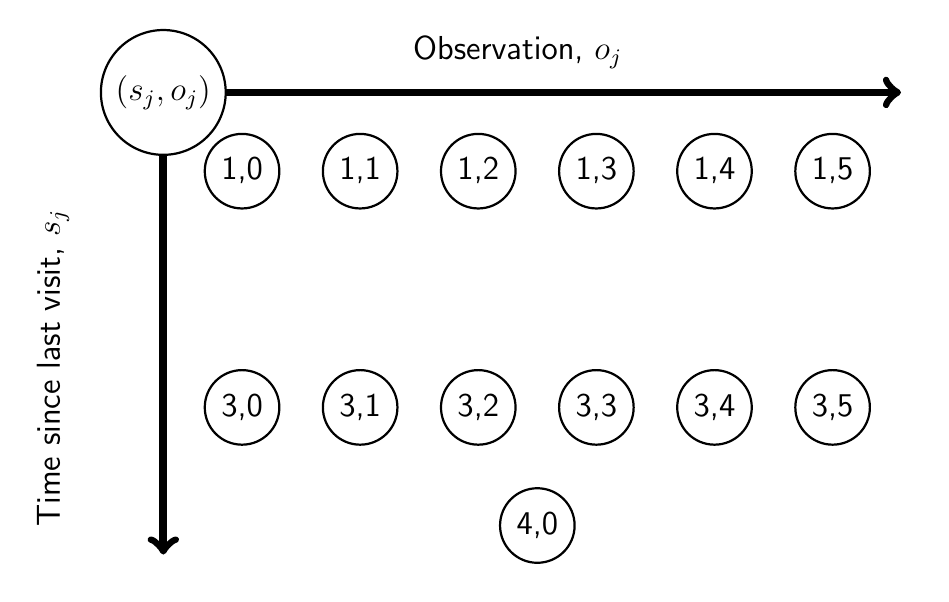
\begin{tikzpicture}[-,auto,node distance=1cm,
                    thick,main node/.style={circle,fill=white,draw,font=\sffamily\large,minimum size=0.5cm}]
 \foreach \x in {0,...,5}
    \foreach \y in {0,2} 
       {\pgfmathtruncatemacro{\label}{\x - 5 *  \y +21}
        \pgfmathtruncatemacro{\o}{\x}
        \pgfmathtruncatemacro{\s}{3-\y}
       \node [main node]  (\x\y) at (1.5*\x,1.5*\y) {\s,\o};}
       
\node[main node] (SpecialState) at (3.75,-1.5) {4,0};       

\node (XaxisLeft) [shift={(-0.5,1)}] at (02) {};
\node (XaxisRight) [shift={(1,1)}] at (52) {};

\node (YaxisBottom) [shift={(-1,-0.5)}] at (0,-1.5) {};
\node (YaxisTop) [shift={(-1,1)}] at (02) {};

\draw[->,line width=1mm] (XaxisLeft)--(XaxisRight);
\draw[->,line width=1mm] (YaxisTop)--(YaxisBottom);

\node[font=\sffamily\large] (OLabel) [shift={(0.5,1.5)}] at (22) {Observation, $o_{j}$};
\node[font=\sffamily\large] (SLabel) [shift={(-2.4,0.5)}] at (00) {\rotatebox{90}{Time since last visit, $s_{j}$}};

\node[main node] (Example) [shift={(-1,1)}] at (02) {$(s_{j},o_{j})$};

\end{tikzpicture}
\end{center}
\caption{Bernoulli with $b_{j}=5$, $x_{1,j}=3.1$ and $x_{2,j}=1.1$}
\end{myfigure}

We will be assuming that $\floor{x_{1}} \neq \floor{x_{2}}$ as otherwise it follows that only one $s_{j}$ survives and we fall into the deterministic category (bar some changes to the values) see Apendix \ref{Bernoulli Attack time with equal floors}.

Suppose we are in the state $(\floor{x_{1}}+1,o)$ for some $o=1,2,...,b$ then our decision is either to
\begin{itemize}
\item Visit now
\item Wait till we are in state $(\floor{x_{2}}+1,o)$ and then visit
\item Wait till we are in state $(\floor{x_{2}}+2,o)$ and then visit
\item Wait till we are in state $(\floor{x_{2}}+2,o)$ and wait
\end{itemize}

Now we write down the long-run average costs of following such a strategy
\begin{itemize}
\item Visit now:
\begin{equation}
\frac{c \lambda \int_{0}^{\floor{x_{1}}} P(X \leq t)dt +\omega}{\floor{x_{1}}+1}
=\frac{\omega}{\floor{x_{1}}+1}
\end{equation}
\item Wait till state $(\floor{x_{2}}+1,o)$ and then visit:
\begin{align}
&\frac{c \lambda \int_{0}^{\floor{x_{2}}} P(X \leq t)dt + coP(X \leq \floor{x_{2})})+\omega}{\floor{x_{2}}+1} \nonumber \\&=\frac{c \lambda (\floor{x_{2}}-x_{1})p +cop + \omega}{\floor{x_{2}}+1}
\end{align}


\item Wait till state $(\floor{x_{2}}+2,0)$ and then visit:
\begin{align}
&\frac{c \lambda \int_{0}^{\floor{x_{2}}+1} P(X \leq t)dt +coP(X \leq \floor{x_{2}}+1)+\omega}{\floor{x_{2}+2}} \nonumber \\ &=\frac{c \lambda ((x_{2}-x_{1})p + (\floor{x_{2}}+1-x_{2}))+co+\omega}{\floor{x_{2}}+2}
\end{align}

\item In state $(\floor{x_{2}}+2,0)$ waiting $k \geq 1$ then visiting:
\begin{align}
&\frac{c \lambda \int_{0}^{\floor{x_{2}}+1+k} P(X \leq t)dt +coP(X \leq \floor{x_{2}}+1+k)+\omega}{\floor{x_{2}+2+k}} \nonumber \\ &=\frac{c \lambda ((x_{2}-x_{1})p + (\floor{x_{2}}+1+k-x_{2}))+co+\omega}{\floor{x_{2}}+2+k}
\end{align}

\end{itemize}


Very similar to before we will look at when certain costs are better. Starting with Visit now beating all others if $ \omega < \frac{cp(\floor{x_{1}}+1)(\lambda (\floor{x_{2}}-x_{1})+o)}{\floor{x_{2}}-\floor{x_{1}}}$ and $\omega < \frac{c(\floor{x_{1}}+1)(\lambda (x_{2}-x_{1})p + (\floor{x_{2}}-x_{2}+1)+o)}{\floor{x_{2}}-\floor{x_{1}}+1}$ and $\omega < \frac{c(\floor{x_{1}}+1)(\lambda (x_{2}-x_{1})p + (\floor{x_{2}}-x_{2}+1+k)+o)}{\floor{x_{2}}-\floor{x_{1}}+1+k}$ for all $k \geq 1$. The first inequality guarantees the other two so we get

Visit now if:
\begin{equation}
\omega < \frac{cp(\floor{x_{1}}+1)(\lambda (\floor{x_{2}}-x_{1})+o)}{\floor{x_{2}}-\floor{x_{1}}}
\end{equation}

We can similarly find the visit in state $(\floor{x_{2}}+1,o)$ by requiring that $ \omega > \frac{cp(\floor{x_{1}}+1)(\lambda (\floor{x_{2}}-x_{1})+o)}{\floor{x_{2}}-\floor{x_{1}}}$ and $\omega < c (\lambda ( p( (x_{2}-x_{1})(\floor{x_{2}}+1)-(\floor{x_{2}}-x_{1})(\floor{x_{2}}+2)) + (\floor{x_{2}}-x_{2}+1)(\floor{x_{2}}+1)+o((1-p)(\floor{x_{2}}+1)-p))$ and $\omega < \frac{c}{k+1} (\lambda ( p( (x_{2}-x_{1})(\floor{x_{2}}+1)-(\floor{x_{2}}-x_{1})(\floor{x_{2}}+2+k)) + (\floor{x_{2}}-x_{2}+k+1)(\floor{x_{2}}+1)+o((1-p)(\floor{x_{2}}+1)-p(k+1)))$. Note the second inequality implies the third one, so

Visit in state $(\floor{x_{2}}+1,o)$ if:
\begin{align}
&\frac{cp(\floor{x_{1}}+1)(\lambda (\floor{x_{2}}-x_{1})+o)}{\floor{x_{2}}-\floor{x_{1}}} < \omega < \nonumber \\ &c (\lambda ( p( (x_{2}-x_{1})(\floor{x_{2}}+1)-(\floor{x_{2}}-x_{1})(\floor{x_{2}}+2)) + (\floor{x_{2}}-x_{2}+1)(\floor{x_{2}}+1)+o((1-p)(\floor{x_{2}}+1)-p)) \nonumber \\
&=c (\lambda (1-p)((\floor{x_{2}}-x_{2})(\floor{x_{2}}+1) + \floor{x_{2}}) + 1 +px_{1} +o((1-p)(\floor{x_{2}}+1)-p))
\end{align}

Again we could possible not have this region if the left hand side overlaps the right (but for now we will ignore it).

Again we can similarly find the visit in state $(\floor{x_{2}}+2,0)$ by requiring that
$ \omega > \frac{cp(\floor{x_{1}}+1)(\lambda (\floor{x_{2}}-x_{1})+o)}{\floor{x_{2}}-\floor{x_{1}}}$ and $\omega > c (\lambda ( p( (x_{2}-x_{1})(\floor{x_{2}}+1)-(\floor{x_{2}}-x_{1})(\floor{x_{2}}+2)) + (\floor{x_{2}}-x_{2}+1)(\floor{x_{2}}+1)+o((1-p)(\floor{x_{2}}+1)-p))$ and $\omega < c (\lambda (1+E[X])-o)$. Now the second inequality implies the first one (???? double check this ????), so

Visit in state $(\floor{x_{2}}+2,0)$ immediately if:
\begin{align}
&c (\lambda (1-p)((\floor{x_{2}}-x_{2})(\floor{x_{2}}+1) + \floor{x_{2}}) + 1 +px_{1} +o((1-p)(\floor{x_{2}}+1)-p)) \nonumber \\
&< \omega < c(\lambda (1+E[X])-o)
\end{align}

Again there is a possibility of overlap (but for now we will ignore it)

Finally we will never visit if:
\begin{equation}
\omega > c(\lambda (1+E[X])-o)
\end{equation}


\begin{example}
Suppose $x_{1}=0.1$,$x_{2}=2.1$ with $p=0.2$ and $b=5$, then our state space is reduced to $\Omega= \{ (1,o) \, | o=0,1,...,5 \} \cup \{ (1,o) \, | o=0,1,...,5 \} \cup \{ (4,0) \}$ and we make the decision at state $(1,o)$. We start by calculating the various critical regions, for which we will use $\lambda=20$ and $o=1$.

First critical value(Equation 12): $\frac{c(0+1)(20 \times (2-0.1)+1)}{2-0}=\frac{39c}{2}=19.5c$

Second critical value(Equation 13): $c(20 \times (1-0.2)((2-2.1)(2+1)+1)+1+0.2 \times 0.1 + 1 \times ((1-0.2)(2+1)-0.2))=14.42c$

Third critical value(Equation 14): $c(20 \times (1+ 0.2 \times 0.1+0.8 \times 2.1)-1)=53c$.

So in this case the decision will be based on the cost, $\omega$:
\begin{itemize}
\item Visit immediately if $\omega \leq 19.5c$
\item Wait till $(4,0)$ (three time periods) and visit immediately if $19.5c <\omega < 53c$
\item Never visit if $\omega \geq 53c$
\end{itemize}
\end{example}

\subsection{Correction to approach for bernoulli}
We will first have a concrete argument as to why we can renew all states, $(s,v)$ with $s < \floor{x_{1}}+1$. From this position consider the policy which waits $k$ time periods and then renews and follows the optimally policy, $\sigma$, with $k=0,...,\floor{x_{1}}+1-s$.

Using such a policy will get us that
\begin{equation}
V_{n}^{\pi_{k}}(s,v)=\omega+E[V_{n-k-1}^{\sigma}(\theta)]
\end{equation}
Where $\theta$ is the state upon renewal (i.e the state $(1,V) \sim (1,TPo(\lambda)$)

Now we will pick policy $\pi_{k+1}$ over $\pi_{k}$ (or be indifferent) if

\begin{align*}
&\lim\limits_{n \rightarrow \infty} V_{n}^{\pi_{k}} (s,v) - V_{n}^{\pi_{k+1}}(s,v) \geq 0 \\
& \iff \lim\limits_{n \rightarrow \infty} E[V_{n-k-1}^{\sigma}(\theta) - V_{n-k-2}^{\sigma} (\theta)] \geq 0 \\
& \iff g \geq 0
\end{align*}

Where $g$ is the average long-run costs of the system, coming from $V_{n}=ng+\phi(s,v)$ for large n, where $\phi(s,v)$ is some initial bias for not starting in the equilibrium but from the initial state $(s,v)$.

Now as the Dynamic Programming only have positive costs, it is impossible for $g < 0$. So we have $g \geq 0 $, so it is better to pick policy $\pi_{k+1}$ over $\pi_{k}$ , as the argument holds for all $k=0,...,\floor{x_{1}}+1-s$ (and all $v$) it is best to wait till $(\floor{x_{1}}+1,v)$ before making a decision, i.e if we are too renew we might as well renew at $(\floor{x_{1}}+1,v)$ (though we might not renew here).

This formally shows the removal of the initial section of states (i.e those at the top).

Now we will skip to the state $(\floor{x_{2}}+2,0)$ and again suggest a policy, $\pi_{k}$ which waits $k$ time periods before renewing and then follows some optimal policy, $\sigma$.

Using such as policy will get us
\begin{align*}
V_{n}^{\pi_{k}}(s,v)&=\omega + c \lambda p  k + c \lambda (1-p) k + E[V_{n-k-1}^{\sigma}(\theta)] \\
&=\omega + c \lambda k + E[V_{n-k-1}^{\sigma}(\theta)] 
\end{align*}

so we will pick policy $\pi_{k+1}$ over $\pi_{k}$ (or be indifferent) if

\begin{align*}
&\lim\limits_{n \rightarrow \infty} V_{n}^{\pi_{k}}(s,v) - V_{n}^{\pi_{k+1}}(s,v) \geq 0 \\
& \iff \lim\limits_{n \rightarrow \infty} -c \lambda + E[V_{n-k-1}^{\sigma}(\theta) - V_{n-k-2}^{\sigma} (\theta)] \\
& \iff -c \lambda + g \geq 0 \\
& \iff f \geq c \lambda
\end{align*}

So hence if $g \geq c \lambda$ we will wait forever, as this has no dependence on $k$.

We will now argue that $g_{\text{max}}= c \lambda$, that is the worst long-run average cost is $c \lambda$. This can be be seen by the strategy, $\pi_{\text{neg}}$, a strategy which never renews no matter what state we are in. I.e the patroller neglects the node. We will have that, for large $n$

\begin{align*}
V_{n}^{\pi_{\text{neg}}}(s,v)= n c \lambda + \phi(s,v)
\end{align*}
We can observe this by looking at the actual decay of the process under a policy that never renews

\begin{align*}
V_{n}^{\pi_{\text{neg}}}(s,v)&= \begin{cases}
n c \lambda \text{ If } s \geq \floor{x_{2}}+2 \\
V_{n-(\floor{x_{2}}+2-s)} + \phi(s,v) \text{ If }  s \leq \floor{x_{2}}+1
\end{cases} \\
&= \begin{cases}
n c \lambda \text{ If } s \geq \floor{x_{2}}+2 \\
(n-(\floor{x_{2}}+2-s)) c \lambda + \phi(s,v) \text{ If }  s \leq \floor{x_{2}}+1
\end{cases} \\
\end{align*}

where

\begin{align*}
\phi(s,v)=&\begin{cases}
\underbrace{v c }_{\text{Observed finishing}} + \underbrace{c \lambda p (\floor{x_{2}}-x_{1}+1)}_{ x_{1} \text{ type attackers finishing}} + \underbrace{c \lambda (1-p) (\floor{x_{1}}-x_{1}+1)}_{ x_{2} \text{ type attackers finishing}} \text{ If } s \leq \floor{x_{1}}+1  \\
\underbrace{v c (1-p)}_{\text{Observed } x_{2} \text{ types finishing}} + \underbrace{c \lambda p (\floor{x_{2}}-x_{1}+1-s)}_{ x_{1} \text{ type attackers finishing}} + \underbrace{c \lambda (1-p) (\floor{x_{1}}-x_{1}+1)}_{ x_{2} \text{ type attackers finishing}} \text{ If } \floor{x_{1}}+2 \leq s \leq \floor{x_{2}}+1 \\
0 \text{ If } s \geq \floor{x_{2}}+2 
\end{cases} \\
&=\begin{cases}
v c + c \lambda (\floor{x_{2}}-x_{2}+1) + c \lambda p (x_{2}-x_{1}) \text{ If } s \leq \floor{x_{1}}+1  \\
v c p + c \lambda (\floor{x_{2}}-x_{2}+1) + c \lambda p (x_{2}-x_{1}-s) \text{ If } \floor{x_{1}}+2 \leq s \leq \floor{x_{2}}+1 \\
0 \text{ If } s \geq \floor{x_{2}}+2 
\end{cases}
\end{align*}

is the `transfer'/bias from the initial state to $(\floor{x_{2}}+2,0)$.

Hence for any service cost, $\omega$ we can achieve a $g= c \lambda$. So we will always be in the case of $g \leq c \lambda$ and hence will renew if we hit the state $(\floor{x_{2}}+2,0)$.

Now in this cases of $g \leq c \lambda$ (where we will not just follow neglection) we need to make a decision about what to do at states $(s,v)$ for $\floor{x_{1}}+1 \leq s \leq \floor{x_{2}}+1$, $0 \leq v \leq b$.

The real question again is how long we wait, before renewal. Let us suppose we are in one of these states $(s,v)$ then we notice that we will have slightly different costs depending which region we are in and how long we wait. We again use $\pi_{k}$ be the policy to wait $k$ ($k=0,1,...,\floor{x_{2}}-\floor{x_{2}}+1$) time units before renewing and then following some optimal policy, $\sigma$.

If we are in $(\floor{x_{1}}+1,v)$ then we will get

\begin{align*}
V_{n}^{\pi_{k}}(\floor{x_{1}}+1,v)&= \begin{cases}
\omega + E[V_{n-k-1}^{\sigma}(\theta)] \text{ If } k=0 \\
\omega + v c p + c \lambda p (\floor{x_{1}}-x_{1}+1+(k-1)) + E[V_{n-k-1}^{\sigma}(\theta)] \text{ If } 1 \leq k \leq \floor{x_{2}}-\floor{x_{1}} \\
\omega+ vc + c \lambda p (\floor{x_{1}}-x_{1}+1+\floor{x_{2}}-\floor{x_{1}}) + c \lambda (1-p) (\floor{x_{2}}-x_{2}+1) + E[V_{n-k-1}^{\sigma}(\theta)] \text{ If } k= \floor{x_{2}}-\floor{x_{1}}+1
\end{cases} \\
&=\begin{cases}
\omega + E[V_{n-1}^{\sigma}(\theta)] \text{ If } k=0 \\
\omega + v c p + c \lambda p (\floor{x_{1}}-x_{1}+1+(k-1)) E[V_{n-k-1}^{\sigma}(\theta)] \text{ If } 1 \leq k \leq \floor{x_{2}}-\floor{x_{1}} \\
\omega+ vc + c \lambda p (x_{2}-x_{1}) + c \lambda (\floor{x_{2}}-x_{2}+1) \text{ If } k= \floor{x_{2}}-\floor{x_{1}}+1
\end{cases}
\end{align*}

If we are in $(s,v)$ for $1 \leq s \leq \floor{x_{2}}$

\begin{align*}
V_{n}^{\pi_{k}}(\floor{x_{1}}+1,v)&= \begin{cases}
\omega + c \lambda p k + E[V_{n-k-1}^{\sigma}(\theta)] \text{ If } 0 \leq k \leq \floor{x_{2}}-\floor{x_{1}}-s \\
\omega+ vc(1-p) + c \lambda p (\floor{x_{2}}-\floor{x_{1}}-s+1) + c \lambda (1-p) (\floor{x_{2}}-x_{2}+1) + E[V_{n-k-1}^{\sigma}(\theta)] \text{ If } k= \floor{x_{2}}-\floor{x_{1}}+1-s+1
\end{cases} \\
&=\begin{cases}
\omega + c \lambda p k E[V_{n-k-1}^{\sigma}(\theta)] \text{ If } 0 \leq k \leq \floor{x_{2}}-\floor{x_{1}}-s \\
\omega+ vc(1-p) + c \lambda p (x_{2}-\floor{x_{1}}-s) + c \lambda (\floor{x_{2}}-x_{2}+1) \text{ If } k= \floor{x_{2}}-\floor{x_{1}}-s+1
\end{cases}
\end{align*}

If we are in $(\floor{x_{2}}+1,v)$ 

\begin{align*}
V_{n}^{\pi_{k}}(\floor{x_{2}}+1,v)&= \begin{cases}
\omega + E[V_{n-k-1}^{\sigma}(\theta)] \text{ If } k=0 \\
\omega+ vc(1-p) + c \lambda p + c \lambda (1-p) (\floor{x_{2}}-x_{2}+1) + E[V_{n-k-1}^{\sigma}(\theta)] \text{ If } k= 1
\end{cases} \\
&=\begin{cases}
\omega + E[V_{n-k-1}^{\sigma}(\theta)] \text{ If } k=0 \\
\omega+ vc(1-p) + c \lambda p (x_{2}-\floor{x_{2}}) + c \lambda (\floor{x_{2}}-x_{2}+1) + E[V_{n-k-1}^{\sigma}(\theta)] \text{ If } k= 1
\end{cases}
\end{align*}

We now seek to compare policies for states, we we shall start with the state, $(\floor{x_{2}}+1,v)$ then we will pick policy $\pi_{0}$ over $\pi_{1}$ if

\begin{align*}
&\lim\limits_{n \rightarrow \infty} V_{n}^{\pi_{1}}(\floor{x_{2}}+1,v) - v_{n}^{\pi_{0}} (\floor{x_{2}}+1,v) \geq 0 \\
& \iff \lim\limits_{n \rightarrow \infty} \omega+ vc(1-p) + c \lambda p (x_{2}-\floor{x_{2}}) + c \lambda (\floor{x_{2}}-x_{2}+1) + E[V_{n-2}^{\sigma}(\theta)]-(\omega + E[V_{n-1}^{\sigma}(\theta)]) \\
& \iff \lim\limits_{n \rightarrow \infty} E[V_{n-2}^{\sigma}(\theta)-V_{n-1}^{\sigma}(\theta)] + vc(1-p)+ c \lambda p(x_{2}-\floor{x_{2}}) + c \lambda (\floor{x_{2}}-x_{2}+1) \\
& \iff g \leq vc(1-p)+ c \lambda p(x_{2}-\floor{x_{2}})) + c \lambda (\floor{x_{2}}-x_{2}+1)
\end{align*}

So we will renew immediately in $(\floor{x_{2}}+2,0)$ from here if $ g \leq vc(1-p)+ c \lambda p(x_{2}-\floor{x_{2}})) + c \lambda (\floor{x_{2}}-x_{2}+1) $. We will use $R_{2}=x_{2}-\floor{x_{2}}$ ($0 \leq R_{2} < 1$).

So to have the possibility to wait and renew we will need that $vc(1-p) + c \lambda p R_{2} + c \lambda (1-R_{2}) \leq c \lambda \iff c(1-p)(v-R_{2} \lambda) \leq 0 \iff v- R_{2} \lambda \leq 0 \iff v \leq R_{2} \lambda$.

\begin{note}
We note that this sort of result is analogous to the deterministic case.
\end{note}

now we note that we can again create a $v_{\text{crit}}(\floor{x_{2}}+1)$, from which we will renew immediately for all  $v \geq v_{\text{crit}}(\floor{x_{2}}+1)$ and for $v < v_{\text{crit}}(\floor{x_{2}}+1)$ we wait.

We rearrange $g \geq vc(1-p)+ c \lambda p(x_{2}-\floor{x_{2}})) + c \lambda (\floor{x_{2}}-x_{2}+1)$ to get $v_{\text{crit}}(\floor{x_{2}}+1)=\ceil{\frac{g}{c(1-p)}- \frac{\lambda}{(1-p)} -\lambda R_{2}}$.

We again know that, $g_{\text{max}}= c \lambda$ so we get the maximum $v_{\text{crit}}=\ceil{\frac{c \lambda}{c (1-p)} - \frac{\lambda}{(1-p)}- \lambda R_{2}}=\ceil{\lambda R_{2}}$

So when $R_{2}=0$ then we immediately renew and will never wait in the state $(\floor{x_{2}}+1,v)$ for any $v$.


\section{Ideas for future}
\begin{itemize}
\item Extend $X$ to be a binomial distribution
\item Extend $X$ to be any discrete distribution
\item Extend $X$ to be a normal distribution by approximation to binomial
\item Test Deterministic case against strategic attacker (non-random) on extended star graph
\end{itemize}
%End of main part of document
\bibliography{mybib}

\appendix
\pagenumbering{roman}
\appendixpage
\addappheadtotoc
\section{Observations are always zero}
\label{Observations are always zero}

On a single node we are limited to the state space of $\Omega=\{ (1,0),...,(\floor{B}+2,0) \}$, then on this state space we can implement a policy which returns every $k$ time units, this will gives an average long run cost of

\begin{equation}
f(k)=\frac{c \lambda \int_{0}^{k-1} P(X \leq t) dt +\omega}{k}
\end{equation}

So to find out when the patroller would be indifferent from choosing to return every $k$ or every $k+1$, solve $f(k+1)-f(k)=0$ giving

$$\frac{1}{k(k+1)}(c \lambda (k \int_{k-1}^{k} P(X \leq t) dt - \int_{0}^{k-1} P(X \leq t) dt ) -\omega)=0 $$

Prompting an index of

$$W(k)=c \lambda (k \int_{k-1}^{k} P(X \leq t) dt - \int_{0}^{k-1} P(X \leq t) dt )$$

We note that $W(0)=0$ and for $k \geq B+1$ $W(k)=c \lambda (k - int_{0}^{k+1} P(X \leq t)dt=c \lambda (1+\int_{0}^{k-1} P(X > t)dt)=c \lambda (1+ E[X])$. We will now show that:
\begin{itemize}
\item $W(k)$ is non-decreasing
\item The optimal policy when $\omega \in [W(k-1),W(k)]$ is to visit every k time units
\item If $w \geq c \lambda (1+E[X])$ then it is optimal to never visit
\end{itemize}

\begin{proof}
First
\begin{align*}
W(k+1)-W(k)&= c \lambda ((k+1) \int_{k}^{k+1} P(X \leq t)dt - \int_{0}^{k} P(X \leq t)dt \\ & \quad \quad \quad -(k \int_{k-1}^{k} P(X \leq t)dt - \int_{0}^{k-1} P(X \leq t)dt)) \\ &=c \lambda ((k+1) \int_{k}^{k+1} P(X \leq t)dt -k \int_{k-1}^{k} P(X \leq t)dt - \int_{k}^{k-1} P(X \leq t)dt)\\ &=c \lambda (k+1) (\int_{k}^{k+1} P(X \leq t)dt - \int_{k-1}^{k} P(X \leq t)dt) \geq 0
\end{align*}

As $P(X \leq t)$ is non-decreasing.

Second if $\omega \in [W(k-1),W(k)]$ then we will show that $f(m)$ is non-increasing for $m \leq k$ and non-decreasing for $m \geq k$.

For $m \leq k$
\begin{align*}
f(m)-f(m-1)&=\frac{1}{m(m-1)}(c \lambda (m-1) \int_{0}^{m-1} P(X \leq t) dt - c \lambda m \int_{0}^{m-2} P(X \leq t) dt - \omega) \\
&=\frac{1}{m(m-1)}(W(m-1)-\omega) \leq \frac{1}{m(m-1)} (W(m-1)-W(k-1)) \leq 0
\end{align*}

Similarly for $m \geq k$
\begin{align*}
f(m+1)-f(m)&= \frac{1}{m(m+1)} (W(m)-\omega) \geq \frac{1}{m(m+1)} (W(m)-W(k)) \geq 0
\end{align*}
Hence choosing to visit every $k$ time units is optimal.

Third and finally our upper limit of $c \lambda (1+E[X])$ (Which is $W(k)$ for $k \geq B+1$) means we are indifferent from picking $k$ and $k+1$ for $k \geq B+1$ so we will never visit. I.e
$f(k+1) \leq f(k) \iff w \geq W(k)$ so not optimal if $f(k+1) \geq f(k) \, \forall k \iff w \geq \sup\limits_{k=1,2,...} W(k)=\lim\limits_{k \rightarrow \infty} W(k)=c \lambda (1+E[X])$
\end{proof}

\section{Bernoulli Attack time with equal floors}
\label{Bernoulli Attack time with equal floors}

If we have $\floor{x_{1}}=\floor{x_{2}}$ then $\Omega= \{(\floor{x_{1}}+1,o) \, | \, o=0,1,...,b \} \cup \{(\floor{x_{1}}+2,o) \}$

Suppose we are in the state $(\floor{x_{1}}+1,o)$ for some $o=1,2,...,b$ then our decision process is the same as the deterministic case
\begin{itemize}
\item Visit now
\item Wait till we are in state $(\floor{x_{1}}+2,0)$ and wait for $k$ time units before visiting, $k \geq 0$
\end{itemize}

We again write down long-run average costs of following such a strategy
\begin{itemize}
\item Visit now:
\begin{equation}
\frac{c \lambda \int_{0}^{\floor{x_{1}}} P(X \leq t) dt + \omega}{\floor{x_{1}}+1}=\frac{\omega}{\floor{x_{1}}+1}
\end{equation}
\item Wait till state $(\floor{x_{1}}+2,0)$ then wait $k \geq 0$ time units before visiting:
\begin{align}
&\frac{c \lambda \int_{0}^{\floor{x_{1}}+1+k} P(X \leq t) dt + coP(X \leq \floor{x_{1}}+1+k) +\omega }{\floor{x_{1}}+2+k} \nonumber \\ &=\frac{c \lambda (p(x_{2}-x_{1})+(\floor{x_{1}}+1+k-x_{2})) + co + \omega}{\floor{x_{1}}+2+k}
\end{align}
\end{itemize}

Now to visit now we will only do so if $\omega < c (\floor{x_{1}}+1) (\lambda (p\frac{x_{2}-x_{1}}{k+1}+ (\frac{\floor{x_{1}}-x_{2}}{k+1} +1))+\frac{o}{k+1})$ for all $k \geq 0$, We need to know if $\lambda (\floor{x_{1}}-px_{1}+px_{2}-x_{2})+o \begin{cases}
 >0 \\
 <0
\end{cases}$. 
In the first case we get to visit if:
\begin{equation}
\omega < c(\floor{x_{1}}+1)(\lambda (\floor{x_{1}}-px_{1}+px_{2}-x_{2}+1)+ o)
\end{equation}
In the second case we get to visit if:
\begin{equation}
\omega < c \lambda (\floor{x_{1}}+1)
\end{equation}



If we do no visit initially then we will visit once transitioned and waited $k+1$ over $k$ if $\omega > c (\lambda (1+E[X])-o)$.

For in between values (dependent on which case) we will get that we will transition and visit immediately.
I.e if
First case
\begin{equation}
c(\floor{x_{1}}+1)(\lambda (\floor{x_{1}}-px_{1}+px_{2}-x_{2}+1)+ o) < \omega < c (\lambda (1+E[X])-o) 
\end{equation}
Second case
\begin{equation}
c \lambda (\floor{x_{1}}+1) < \omega < c (\lambda (1+E[X])-o)
\end{equation}

Again these regions may or may not exist dependent on their conditions.

\end{document}
